\label{sec:dir_energy_fitting_noise}

\begin{figure}[t]
\centering

\begin{subfigure}{0.48\columnwidth}
    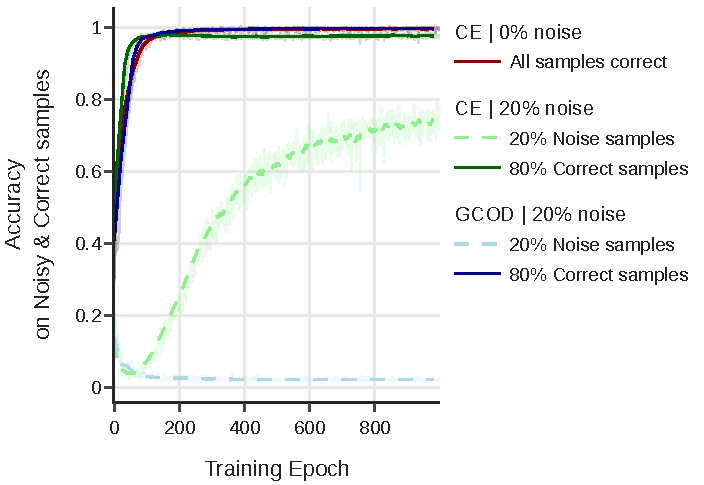
\includegraphics[width=\linewidth]{AISTATS/figures/fig8a}
    \caption{}
    \label{fig:PPA_DE_NCOD_subfig1}
\end{subfigure}
\hfill
\begin{subfigure}{0.48\columnwidth}
    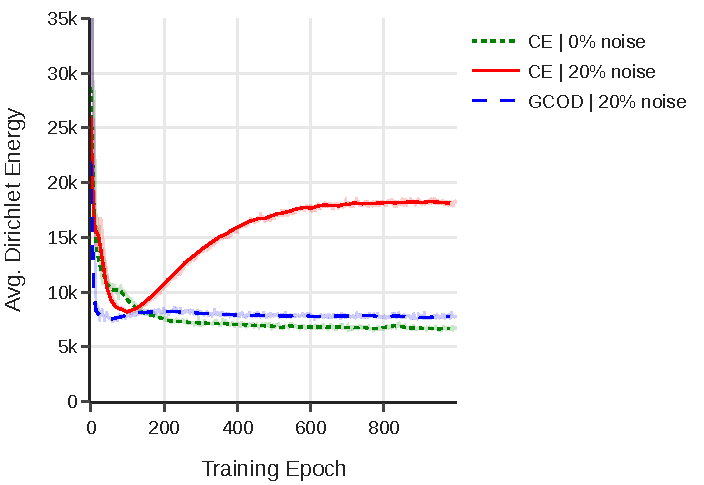
\includegraphics[width=\linewidth]{AISTATS/figures/fig8b}
    \caption{}
    \label{fig:PPA_NCOD_Dirich_energy}
\end{subfigure}

\caption{
(a) Evolution of training Accuracy for GIN model on the PPA dataset (30\% sample, 6 classes) with clean 0\% or 20\% label noise for CE and \method. 
(b) Dirichlet energy for clean and noise introduced PPA dataset (30\% sample, 6 classes). The Dirichlet energy increases when the model with CE fits on noise.
}
\label{fig:dirichlet_results}

\end{figure}


\begin{figure}[t]
\centering

\begin{subfigure}{0.48\columnwidth}
    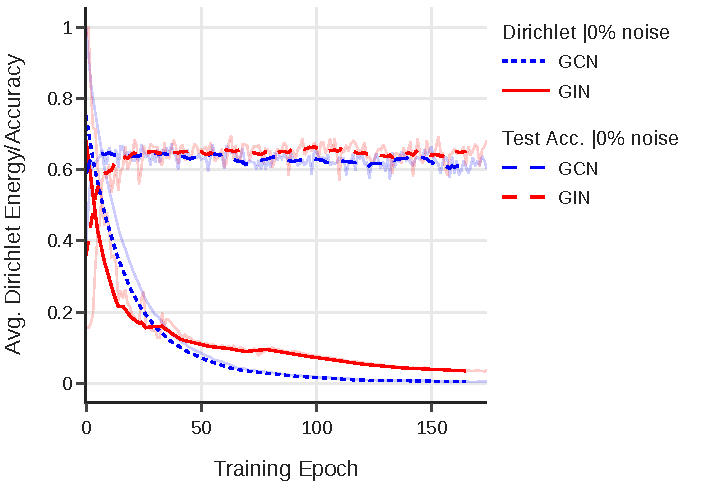
\includegraphics[width=\linewidth]{AISTATS/figures/gin_gcn_dir.pdf}
    \caption{}
    \label{fig:gin_gcn_dir}
\end{subfigure}
\hfill
\begin{subfigure}{0.48\columnwidth}
    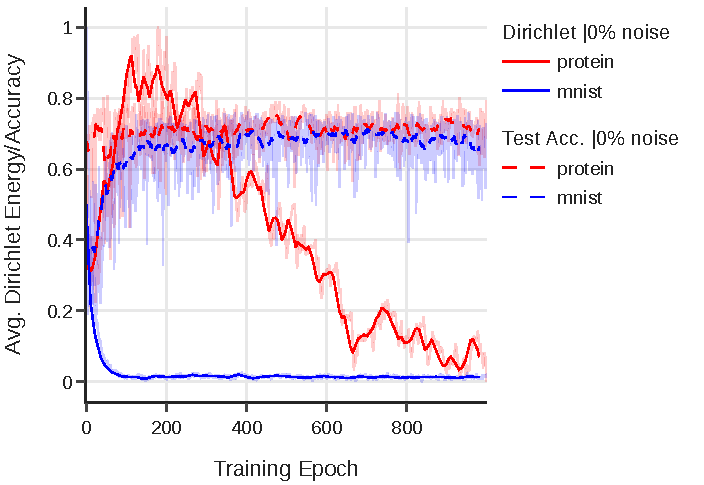
\includegraphics[width=\linewidth]{AISTATS/figures/compareDataset.pdf}
    \caption{}
    \label{fig:comparedataset}
\end{subfigure}

\caption{
(c) Dirichlet energy and test Accuracy on the PPA dataset using CE with GIN and GCN models.
(d) Dirichlet energy and test Accuracy on different datasets using GIN model (axes scaled for comparison).
}
\label{fig:dircihlet_results1}

\end{figure}


% Section~\ref{sec:failure} established that GNNs can overfit noisy labels when model capacity exceeds task requirements. We now investigate \emph{how} this overfitting manifests in learned representations, revealing Dirichlet energy as a reliable diagnostic signal that also suggests intervention strategies.

% Across all experimental setups, we consistently observe that the Dirichlet energy (\(E^{\text{dir}}\)) of the learned node representations increases once the model begins to fit on noisy labels (see Fig. \ref{fig:PPA_NCOD_Dirich_energy}). During early training, when the model captures true patterns, (\(E^{\text{dir}}\)) remains low; however, as the model starts fitting the noisy samples, the energy increases significantly. This consistent behavior across diverse datasets and conditions ( Fig. \ref{fig:PPA_NCOD_Dirich_energy} 
%  and Figure \ref{fig:dirichlet_energy_comparison})  motivates us to use \(E^{\text{dir}}\) as a signal to detect and monitor overfitting to label noise.

% %This empirical observation aligns with theoretical understanding of GNNs. The learnable weight matrices in GNN layers determine whether features are smoothed across the graph  or sharpened. Sharpening directly increases the Dirichlet energy \cite{zhou2021dirichlet}.
% %We conjecture that training on noisy labels, especially those creating false distinctions between similar graphs, forces the model to amplify high-frequency differences to fit these contradictory signals. This process increases the signal's high-frequency content and Dirichlet energy, enabling the model to fit the noise.

% This leads to our first research question \textbf{RQ1}:\textit{ Is Dirichlet energy related to GNN performance on graph classification tasks, and how does it evolve when label noise is introduced during training?} 

% To address this, we propose a graph-level Dirichlet energy measure for the graph classification task and analyze its empirical behavior during training under noise conditions.
% Given a set of graphs $\mathcal{S}$, composed of graphs $\mathcal{G}^i$ with latent representation $\mathbf{Z}^i$, we define the Dirichlet energy of the set $\mathcal{S}$ as
% \begin{equation}
%     \label{eq: avg_dirichlet}
%    E^{dir}_{\text{set}}(\mathcal{S}) := \frac{1}{|\mathcal{S}|} \sum_{\mathcal{G}^i \in \mathcal{S}}  E^{dir}(\mathbf{Z}^i).
% \end{equation}


% In particular, we study $E^{dir}_\text{set}(\mathcal{D}_c)$, the average Dirichlet energy of graphs belonging to class $c$, where $\mathcal{D}_c$ denotes the subset of training graphs with the label $c$. 


% Our empirical analysis provides a consistent answer to \textbf{RQ1}. In clean datasets, i.e., without label noise, \( E^{dir}_{\text{set}}(\mathcal{D}_c) \) may fluctuate during the initial training phase as the model begins to adjust to the task. However, we consistently observe a steady decrease in the later stages of training, culminating in low and stable Dirichlet energy values once the model converges to high classification accuracy. This behavior is illustrated in Fig.~\ref{fig:gin_gcn_dir} and Fig. \ref{fig:comparedataset} for models trained with standard Cross-Entropy (CE) loss and no label noise (CE-0\%).

% However, when synthetic label noise is introduced (e.g., 20\% symmetric flipping), the behavior diverges. As shown in Fig.~\ref{fig:PPA_DE_NCOD_subfig1}, while the initial phase of training still exhibits a decrease in \( E^{dir}_{\text{set}}(\mathcal{D}_c) \), this is followed by a significant increase during later epochs, precisely when the model starts to fit the noisy labels. This memorization phase is marked by rising training accuracy on noisy samples (see CE-20\%), demonstrating a direct link between noise fitting and increased Dirichlet energy.
% This phenomenon is consistently observed across datasets and model architectures, including MUTAG, MNIST, and PROTEINS (see 
% Fig. \ref{fig:comparedataset} and Fig. \ref{fig:mutag} in Appendix \ref{appendix:additional_figures}). These findings confirm that Dirichlet energy serves as a reliable signal of representation smoothness and its disruption as a result of noise memorization.

% Furthermore, to isolate the spectral dynamics, we utilize the HLFF-GNN framework \cite{hlffgnn}, which decomposes the node representations into low-frequency \( \mathbf{Z}_1 \) and high-frequency \( \mathbf{Z}_2 \) components. Experiments show that while \( E^{dir}(\mathbf{Z}_1) \) remains stable, \( E^{dir}(\mathbf{Z}_2) \) sharply increases during noise overfitting, confirming that high frequency energy components are responsible for fitting mislabeled data (detailed analysis of these experiments is provided in Appendix \ref{sec:Amplification}).

% From these observations, we conclude that maintaining a low Dirichlet energy, particularly by suppressing some high-frequency components, correlates with robust generalization. However, directly minimizing \( E^{dir}_{\text{set}}(\mathcal{S}) \) as a loss term presents practical challenges. First, the asymptotic energy level varies between datasets and architectures, making it difficult to define a universal target. Second, \( E^{dir}_{\text{set}} \) is a global dataset level quantity, which is not easily decomposed into sample gradients for stochastic optimization. We propose alternative strategies to promote smoothness. 


Section~\ref{sec:failure} established that GNNs can overfit noisy labels when model capacity exceeds task requirements. We now investigate how this overfitting manifests in learned representations, revealing Dirichlet energy as a reliable diagnostic signal that also suggests intervention strategies.

Across all experimental setups, we consistently observe that the Dirichlet energy (\(E^{\text{dir}}\)) of the learned node representations increases once the model begins to fit on noisy labels (see Fig. \ref{fig:PPA_NCOD_Dirich_energy}). During early training, when the model captures true patterns, (\(E^{\text{dir}}\)) remains low; however, as the model starts fitting the noisy samples, the energy increases significantly. This consistent behavior across diverse datasets and conditions ( Fig. \ref{fig:PPA_NCOD_Dirich_energy} 
 and Figure \ref{fig:dirichlet_energy_comparison})  motivates us to use \(E^{\text{dir}}\) as a signal to detect and monitor overfitting to label noise. This leads to our first research question \textbf{RQ1}:\textit{ Is Dirichlet energy related to GNN performance on graph classification tasks, and how does it evolve when label noise is introduced during training?} 

To address this, we propose a graph-level Dirichlet energy measure for the graph classification task and analyze its empirical behavior during training under noise conditions.
Given a set of graphs $\mathcal{S}$, composed of graphs $\mathcal{G}^i$ with latent representation $\mathbf{Z}^i$, we define the Dirichlet energy of the set $\mathcal{S}$ as
\begin{equation}
    \label{eq: avg_dirichlet}
   E^{dir}_{\text{set}}(\mathcal{S}) := \frac{1}{|\mathcal{S}|} \sum_{\mathcal{G}^i \in \mathcal{S}}  E^{dir}(\mathbf{Z}^i).
\end{equation}
In particular, we study $E^{dir}_\text{set}(\mathcal{D}_c)$, the average Dirichlet energy of graphs belonging to class $c$, where $\mathcal{D}_c$ denotes the subset of training graphs with the label $c$. 

Our empirical analysis provides a consistent answer to \textbf{RQ1}. In clean datasets, i.e., without label noise, \( E^{dir}_{\text{set}}(\mathcal{D}_c) \) may fluctuate during the initial training phase as the model begins to adjust to the task. However, we consistently observe a steady decrease in the later stages of training, culminating in low and stable Dirichlet energy values once the model converges to high classification accuracy. This behavior is illustrated in Fig.~\ref{fig:gin_gcn_dir} and Fig. \ref{fig:comparedataset} for models trained with standard Cross-Entropy (CE) loss and no label noise (CE-0\%).
\looseness=-1

However, when synthetic label noise is introduced (e.g., 20\% symmetric flipping), the behavior diverges. As shown in Fig.~\ref{fig:PPA_DE_NCOD_subfig1}, while the initial phase of training still exhibits a decrease in \( E^{dir}_{\text{set}}(\mathcal{D}_c) \), this is followed by a significant increase during later epochs, precisely when the model starts to fit the noisy labels. This memorization phase is marked by rising training accuracy on noisy samples (see CE-20\%), demonstrating a direct link between noise fitting and increased Dirichlet energy.

This phenomenon is consistently observed across datasets and model architectures, including MUTAG, MNIST, and PROTEINS (see 
Fig. \ref{fig:comparedataset} and Fig. \ref{fig:mutag} in Appendix \ref{appendix:additional_figures}). These findings confirm that Dirichlet energy serves as a reliable signal of representation smoothness and its disruption as a result of noise memorization.
\paragraph{Why Smooth Representations Resist Noisy Graph Labels.}
This connection between smoothness and robustness admits an intuitive explanation specific to graph classification. 
In this setting, graph-level predictions are obtained by pooling node representations (e.g., via mean or sum pooling). 
For correctly labeled graphs, the GNN learns node representations that, when pooled, produce features characteristic of their class—and message passing naturally makes these representations smooth across neighbors.
%
Now consider a mislabeled graph: to fit this incorrect label, the pooled representation must resemble graphs from a \emph{different} class. 
Achieving this requires some node representations to deviate from the smooth patterns learned for correctly-labeled graphs—manifesting as sharp, high-frequency components that increase Dirichlet energy.
%
Thus, the smoothness bias inherent in GNN message-passing acts as implicit regularization against noisy \emph{graph} labels: the model can only fit mislabeled graphs by developing costly high-frequency representations, which it does only when capacity permits and training continues long enough.
This explains the U-shaped energy trajectory in Fig.~\ref{fig:PPA_NCOD_Dirich_energy}: energy decreases while learning true patterns, then increases when memorizing noise.

Furthermore, to isolate the spectral dynamics, we utilize the HLFF-GNN framework \cite{hlffgnn}, which decomposes the node representations into low-frequency \( \mathbf{Z}_1 \) and high-frequency \( \mathbf{Z}_2 \) components. Experiments show that while \( E^{dir}(\mathbf{Z}_1) \) remains stable, \( E^{dir}(\mathbf{Z}_2) \)( Appendix Figure~\ref{fig:dirichlet_energy_comparison}) sharply increases during noise overfitting, confirming that high frequency energy components are responsible for fitting mislabeled data (detailed analysis of these experiments is provided in Appendix \ref{sec:Amplification}).

From these observations, we conclude that maintaining a low Dirichlet energy, particularly by suppressing some high-frequency components, correlates with robust generalization. However, directly minimizing \( E^{dir}_{\text{set}}(\mathcal{S}) \) as a loss term presents practical challenges. First, the asymptotic energy level varies between datasets and architectures, making it difficult to define a universal target. Second, \( E^{dir}_{\text{set}} \) is a global dataset level quantity, which is not easily decomposed into sample gradients for stochastic optimization. We propose alternative strategies to promote smoothness.



